% !TEX root = ../main.tex
%
\chapter{Technical Implementation}
\label{sec:system}

\cleanchapterquote{Innovation distinguishes between a leader and a follower.}{Steve Jobs}{(CEO Apple Inc.)}


\section{System Architecture}
\label{sec:system:architecture}

% Technology Stack Rational
% Architecture Diagram & data flow

The architecture followed a standard client server pattern, with the server functioning as a wrapper for the nerfstudio CLI, and the client as a web application.
The server was built using tRPC, a framework for building type-safe APIs in TypeScript.
It was responsible for handling incoming requests from the client, and translating them into commands that the nerfstudio CLI could understand.
Requests from the client were sent to the server using HTTP requests, and in case of an asynchronous operation, the server would update the client on using websockets.

\begin{figure}[htb]
	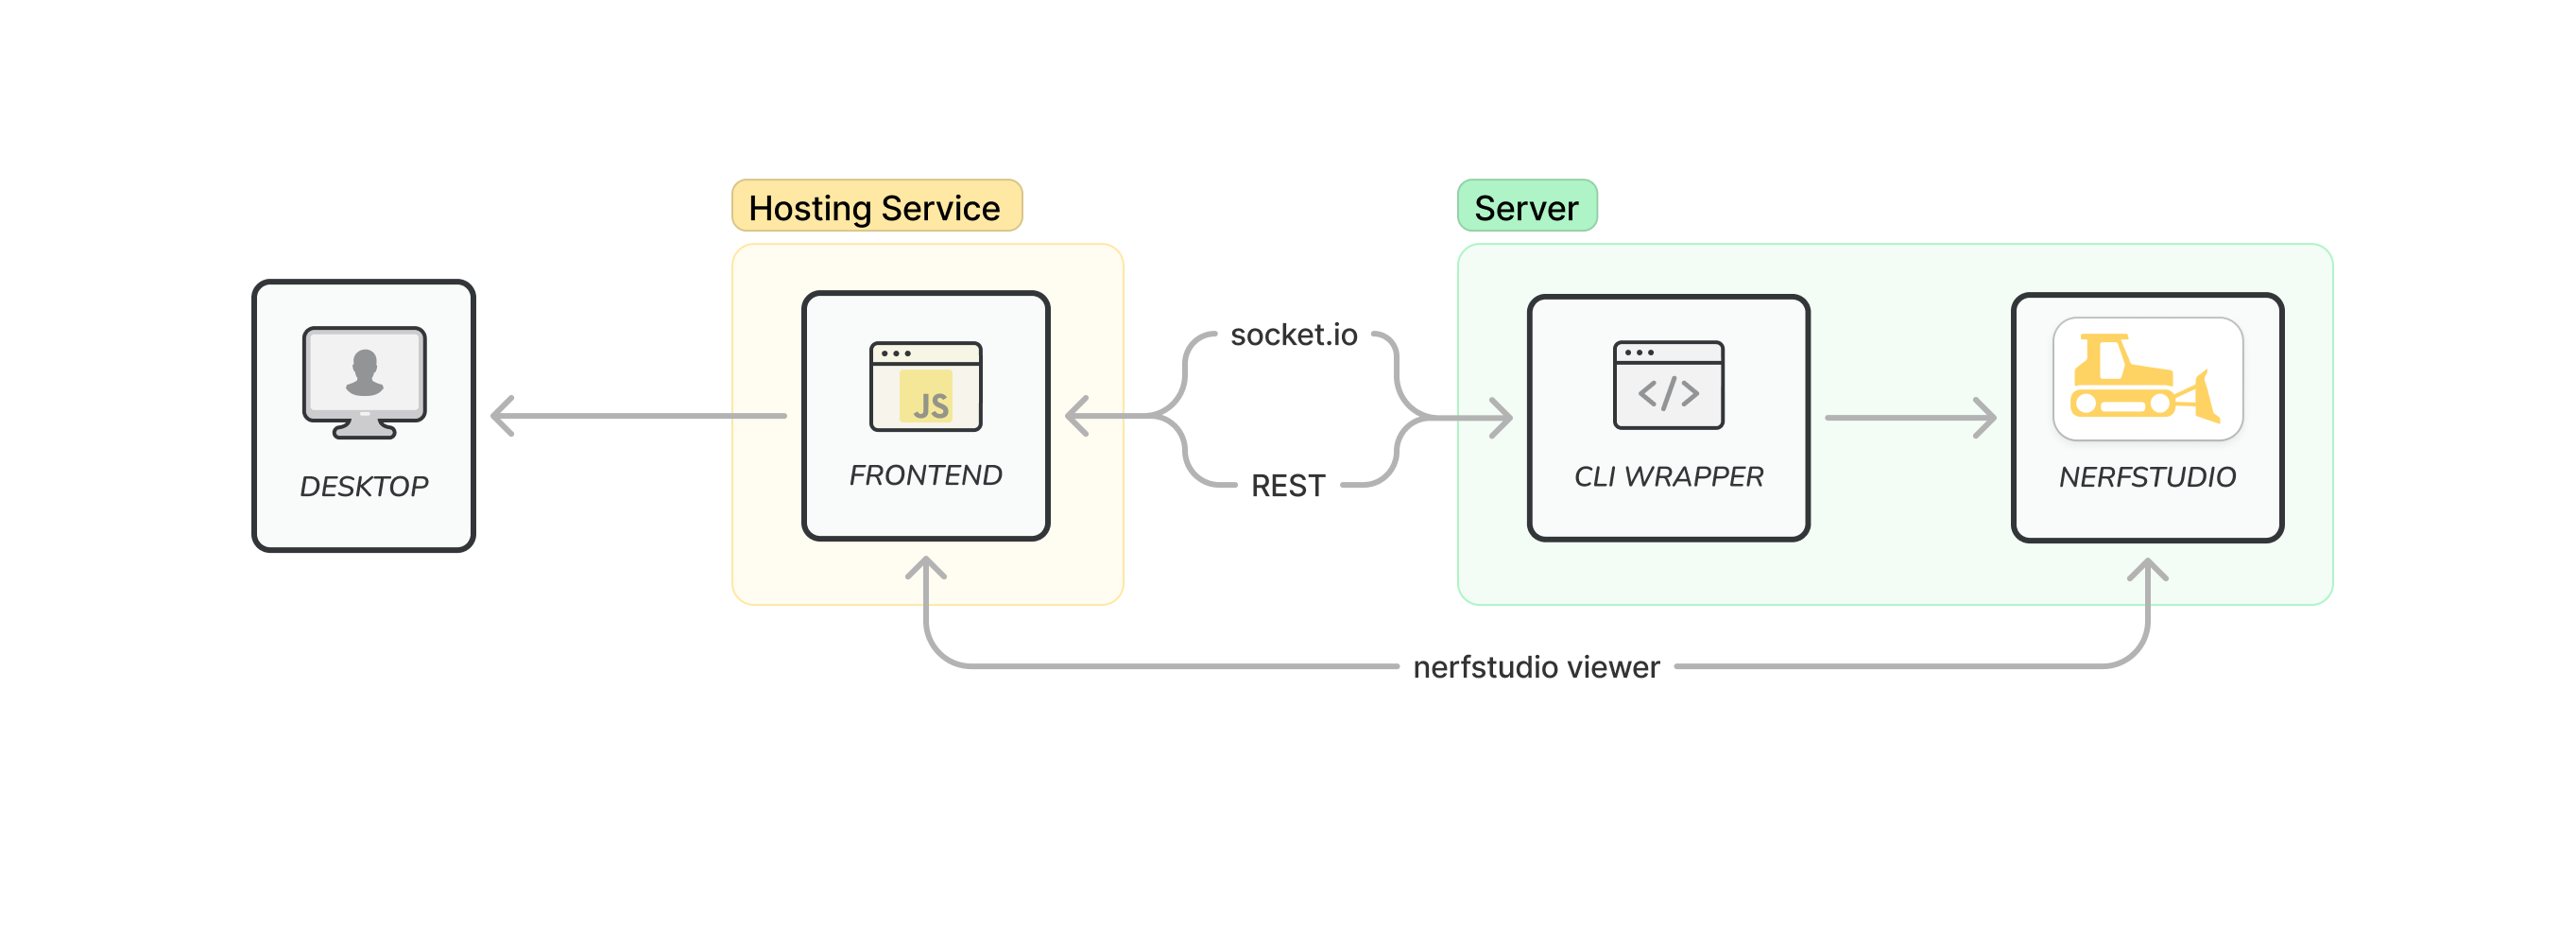
\includegraphics[width=\textwidth]{figures/architecture-1.png}
	\caption{Another Figure example: \textit{(a)} example part one, \textit{(c)} example part two; \textit{(c)} example part three}
	\label{fig:system:example2}
\end{figure}

\section{Frontend Development} 
\label{sec:system:frontend}

% Setup, configuration, and component architecture
% UI/UX design principles


\section{Backend Development}
\label{sec:system:backend}

% Advantages of tRPC, configuration, and API design

\section{Challenges and Solutions}
\label{sec:system:challenges}


\section{Lessons Learned}
\label{sec:system:lessons}

\section{Future Directions}
\label{sec:system:future}
